\chapter{Test d'hypothèses robustes en millieu non-gaussien}
\label{ch:robust-detection}

\section{Introduction}
\label{sec:detection-introduction}


Ce chapitre reprend et reformule, tout en établissant des liens, un ensemble de résultats obtenus aux cours de deux collaborations différentes. 

La première partie concerne la détection multivariée robuste dans un système  SONAR à multiples antennes, dont les résultats ont été obtenus dans la cadre de la thèse d'Olivier Lerda, que j'ai co-dirigé en compagnie de Guillaume Ginolhac et Jean-Philippe Ovarlez. Il s'agit de porter au monde de la détection SONAR les développements de la détection robuste pour les systèmes RADAR à multiples antennes\footnote{On pourra à se sujet se référer aux travaux de la thèse de Chin Yuan Chong \cite{chong:tel-00772006} pour un travail similaire effectué dans le monde RADAR à multiples antennes.}, tout en explorant de nouvelles directions sur la détection basée sur le test de Rao ou bien la détection par sous-espaces.


La deuxième partie concerne une extension de mes travaux de thèse sur la détection de changements en imagerie RSO basées sur des tests d'égalité de matrices de covariances \cite{Mian_2019}. Avec la même équipe qu'à l'époque\footnote{Florent Bouchard et Gauillaume Ginolhac}, nous avons considéré une extension des travaux initiés dans \cite{Bouchard_2020} sur la détection de changements robuste en-ligne dans les séries temporelles d'images RSO. Encore non appliquée en pratique à l'époque, nous avons pu considérer une nouvelle modélisation du problème qui permet de diminuer le nombre de données nécéssaires à l'estimation des paramètres du problèmes, ce qui autorise une application sur données réelles.


\section{Détection multivariée pour une antenne SONAR à croix de Mill's}
\label{sec:detection-mills-antenna}


[Your main content goes here. This is where you'll develop the core ideas and arguments for this chapter.]

\subsection{Contexte et problème de détection}


\subsection{Tests robustes basés sur le GLRT et le test de Rao}


\subsection{Gérer l'incertitude : l'apport des sous-espaces}

You can organize your content using subsections. Some key points to consider:

\begin{itemize}
    \item Point one with relevant details
    \item Point two with supporting evidence
    \item Point three with analysis or discussion
\end{itemize}

\newpage

\section{Détection de changements en-ligne pour les séries temporelles d'images RSO}
\label{sec:detection-online-change-detection}


Phrase de transition sur la partie précédente.... : calculs lourds lié au point-fixe dans l'estimation qui reste un problème dans toutes les méthodes de détection robustes, notamment quand il s'agit d'ajouter des données pour améliorer une estimation précédente. Dans ce contexte, la géométrie riemannienne permet de considérer un cadre d'estimation en ligne basé sur un algorithme de décente de gradient stochastique \cite{Zhou_2019}.

Blabla


\subsection{Problématique de la détection de changements sur matrices de covariances}

Commençons d'abord par introduire la problématique et les limitations pratiques des solutions proposées.

Nous considérons le traitement d'une série temporelle d'images RSO multivariée telle que présentée en Figure \ref{fig:example_its}. Dans ce contexte, chaque pixel correspond à un vecteur $\x\in\C^\vdim$, où $\vdim$ correspond usuellement à une diversité polarimétrique ($\vdim=3$ ou $\vdim=4$ selon les modalités) ou bien spectrale ou encore fréquentielle\footnote{\`A noter que dans la plupart des cas, on n'observe jamais une scène avec un capteur ayant une telle diversité mais avec une image de résolution suffisante, il est possible de constuire des images plus basses résolution ayant cette diversité \cite{Mian_wavelet_2019}.}.

\begin{figure*}
    \begin{tikzpicture}[scale=1]

% -------------------------------------------------
% parameters
% -------------------------------------------------
\pgfmathsetmacro{\cubex}{3}
\pgfmathsetmacro{\cubey}{2}
\pgfmathsetmacro{\cubez}{1}
\pgfmathsetmacro{\wf}{0.45}

% window size
\pgfmathsetmacro{\wx}{\wf*\cubex}
\pgfmathsetmacro{\wy}{\wf*\cubey}

% -------------------------------------------------
% cube drawing macro
% #1 = label index (1 or T)
% -------------------------------------------------
\newcommand{\DrawCube}[1]{

% ---- cube ----
\draw [every edge/.append style={densely dashed, opacity=.5}]
  (0,0,0) coordinate (o) -- ++(-\cubex,0,0) coordinate (a)
  -- ++(0,-\cubey,0) coordinate (b)
  edge coordinate[pos=1] (g) ++(0,0,-\cubez)
  -- ++(\cubex,0,0) coordinate (c) -- cycle
  (o) -- ++(0,0,-\cubez) coordinate (d)
  -- ++(0,-\cubey,0) coordinate (e)
  edge (g) -- (c) -- cycle
  (o) -- (a) -- ++(0,0,-\cubez) coordinate (f)
  edge (g) -- (d) -- cycle;

% ---- face center ----
\coordinate (Fc) at (-0.5*\cubex,-0.5*\cubey,0);

% window corners (robust)
\coordinate (W1) at ($(Fc)+(-\wx/2,\wy/2,0)$);
\coordinate (W2) at ($(Fc)+(\wx/2,-\wy/2,0)$);

% filled window
\fill[gray!20] (W1) rectangle (W2);

% 3x3 grid
% --- outer border ---
\draw (W1) rectangle (W2);

% --- vertical grid lines ---
\foreach \i in {1,2}{
  \draw ($(W1)+(\i*\wx/3,0,0)$) --
        ($(W1)+(\i*\wx/3,-\wy,0)$);
}

% --- horizontal grid lines ---
\foreach \i in {1,2}{
  \draw ($(W1)+(0,-\i*\wy/3,0)$) --
        ($(W1)+(\wx,-\i*\wy/3,0)$);
}


% annotation
\node[above=11pt] at (Fc) {$ \mathcal{X}_{\iobs #1}=\x_{\iobs #1}$};

% time label
\node at (-4,-1,0) {$t=#1$};

}

% -------------------------------------------------
% DRAW BOTH CUBES (HORIZONTAL)
% -------------------------------------------------

\foreach \label/\xshift in {1/0, T/7}{
  \begin{scope}[xshift=\xshift cm]
    \DrawCube{\label}
  \end{scope}
}

% vertical dots
\node at (-1.5,-2.25) {$\dots$};

\end{tikzpicture}


  \vspace{0.5em}
  \caption{Illustration de la dimensionalité de nos données SITS et de la fenêtre sur laquelle on considère les données pour le test de détection. $\x_{\iobs}$ est l'observation de la variable sous-jacente $\Variable_{\iobs\itime}$. }
  \label{fig:slidingwindows}
\end{figure*}



%TODO:: add figures of local neighborhood and global time series examples
%TODO: add citations
Pour effectuer une détection de changements, on se base sur la notion de voisinage spatial au cours du temps $\Xset_t = \{\x_{\iobs\itime}:1\leq \iobs \leq \Nobs\}$ comme illustré à la figure \ref{fig:slidingwindows}. En considérant que la distribution des données $\p{\Variable_{\iobs\itime}}$ est iid sur le voisinage : $\p{\Variable_{\iobs\itime}}(\x_{\iobs\itime})\equiv\p{\Variable_{t}}(\x_{\iobs\itime}),\,\forall \iobs\in\{1,\dots,\Nobs\}$, on peut identifier un changement à cet endroit à travers l'évolution de cette densité au cours du temps : si elle reste constante il n'y a pas eu de changements alors qu'une évolution de celle-ci indique qu'il s'est passé quelque chose. Formellement, on peut définir le problème de détection comme :



\begin{figure*}[t]
  \foreach \i in {1,...,16}{
    \includegraphics[width=0.3\textwidth]{gfx/chapter-detection/sar/sar_its/image_\i.jpg}
  }
  % TODO: find back the reference of image time series
  \caption{Exemple de SITS extraite de données UAVSAR polarimétriques en représentation de Pauli (Rouge: $|x_{\HH}-x_{\VV}|$, Rouge: $|x_{\HV}|$, Rouge: $|x_{\HH}+x_{\VV}|$). Images extraites à l'aide du code disponible à l'adresse: \url{https://github.com/AmmarMian/simulations_hdr/blob/main/2-detection/sar_experiments/visualisations/show_sar_its.py}.}
  \label{fig:example_its}
\end{figure*}

\begin{figure*}[t]
  % This file was created with matplot2tikz v0.5.3.
\begin{tikzpicture}

\definecolor{darkgray176}{RGB}{176,176,176}

\begin{axis}[
width=0.4\linewidth,
height=7cm,
colorbar,
colorbar style={ylabel={}},
colormap/viridis,
point meta max=248.592788696289,
point meta min=1.54258155822754,
tick align=outside,
tick pos=left,
title={$\DetectorStat_\gaussian$ (5.32s)},
x grid style={darkgray176},
xmin=-0.5, xmax=1493.5,
xtick style={color=black},
y dir=reverse,
y grid style={darkgray176},
ymin=-0.5, ymax=2993.5,
ytick style={color=black}
]
\addplot graphics [includegraphics cmd=\pgfimage,xmin=-0.5, xmax=1493.5, ymin=2993.5, ymax=-0.5] {gfx/chapter-detection/sar/detection_results/gaussian_torch-cuda_Scene_3_20260303_110317-000.png};
\end{axis}

\end{tikzpicture}

  % This file was created with matplot2tikz v0.5.3.
\begin{tikzpicture}

\definecolor{darkgray176}{RGB}{176,176,176}

\begin{axis}[
width=0.4\linewidth,
height=7cm,
colorbar,
colorbar style={ylabel={}},
colormap/viridis,
point meta max=14241.62890625,
point meta min=134.353149414062,
tick align=outside,
tick pos=left,
title={$\DetectorStat_\compoundgaussian$ (240.69s)},
x grid style={darkgray176},
xmin=-0.5, xmax=1493.5,
xtick style={color=black},
y dir=reverse,
y grid style={darkgray176},
ymin=-0.5, ymax=2993.5,
ytick style={color=black}
]
\addplot graphics [includegraphics cmd=\pgfimage,xmin=-0.5, xmax=1493.5, ymin=2993.5, ymax=-0.5] {gfx/chapter-detection/sar/detection_results/dcg_torch-cuda_Scene_3_20260303_110339-000.png};
\end{axis}

\end{tikzpicture}

  \vspace{-1em}
  \caption{Sorties de détecteurs sur la SITS présentée en figure \ref{fig:example_its} avec une fenêtre de $\Nobs=7\times 7$. Le nombre d'itérations des points-fixes est fixé à 10.}
  \label{fig:cd_maps}
\end{figure*}



\begin{equation}
  \left\{ \begin{array}{lll} \hypothesis_0: &  \forall \itime, & \p{\Variable_\itime} \equiv \p{\Variable_1}   \\ 
  \hypothesis_1: & \exists (\itime_1, \itime_2)\, / & \p{\Variable_{\itime_1}} \not\equiv  \p{\Variable_{\itime_2}}  \end{array}\right. .
\end{equation}

%TODO : find citations
En pratique, il devient difficile de mettre en place une stratégie de décision à partir de ce modèle sans préciser la distribution à priori des données. En ce sens, tout comme pour les données SONAR vues précédemment, deux modèles existent pour les images RSO: le modèle gaussien multivarié centré pour les images à faible résolution \cite{lee2017polarimetric} et le modèle elliptique centré pour les images à très haute résolution \cite{413444, greco2007statistical}. Dans les deux cas, la distribution étant paramétrique : $\Variable_t \sim p_{\Variable_t}(\x_t;\param_t)$, on peut redéfinir le problème de détection à partir de l'évolution des paramètres du modèle :

\begin{equation}
  \left\{ \begin{array}{lll} \hypothesis_0: &  \forall \itime, & \param_t = \param_1   \\ 
  \hypothesis_1: & \exists (\itime_1, \itime_2)\, / & \param_{t_1} = \param_{\itime_2} \end{array}\right. .
\end{equation}

Dans le cas gaussien, les données étant centrées par construction la détection se fait sur la matrice de covariance : $\param_t = \{\MCov_t\}$, ce qui revient à un problème très connu dans la littérature statistique : le test d'égalité de matrices de covariances \cite{anderson1958introduction}. Le GLRT du problème a été dérivé et se formule comme un rapport de déterminants :
\begin{equation}
  \DetectorStat_\gaussian \propto \dfrac{\Det(\sum_{\itime=1}^{\Ntime} \Smat_\itime)}{\prod_{\itime=1}^{\Ntime} \Det(\Smat_\itime)} \detect .
  \label{eq:glrt_gaussian_cd}
\end{equation}


%TODO: lier à l'équation du modèle CCG en chapitre 1
Dans le cas elliptique, la méconnaissance de la fonction génératrice de densité complique la dérivation d'un détecteur universel. Ainsi, nous avons pu proposer de passer par la modélisation en distribution gaussienne composée : $\param_t = \{\texture_{1\itime},\dots,\texture_{\Nobs\itime}, \MCov\}$. Dans ce cas, le GLRT est tractable et se formule comme \cite{Mian_2019}:
\begin{equation}
  \DetectorStat_\compoundgaussian \propto \dfrac{\Det(\Tyler_0)}{\prod_{\itime=1}^{\Ntime} \Det(\Tyler_t)} \prod_{\iobs=1}^{\Nobs} \dfrac{\sum_{\itime=1}^{\Ntime}\q{\x_{\iobs\itime}}{\Tyler_0}}{\prod_{\itime=1}^{\Ntime}\q{\x_{\iobs\itime}}{\Tyler_t}} \detect,
  \label{eq:glrt_nongaussian_cd}
\end{equation}

où $\Tyler_0$ est une variante de l'estimateur de Tyler, défini comme étant la solution de l'équation de point-fixe:
\begin{equation}
  \Tyler_0 = \frac{\vdim}{\Nobs} \sum_{\iobs=1}^{\Nobs} \dfrac{\sum_{\itime=1}^{\Ntime} \Smat_\itime}{\sum_{\itime=1}^{\Ntime} \q{\x_{\iobs\itime}}{\Tyler_0}}.
\end{equation}

%TODO: make sure that quadratic form q is defined well beforehand
%TODO: Parler des avantages théoriques du détecteur robuste

À titre d'exemple, les résutlat du calcul de ces statistiques sur la séries d'images en figure \ref{fig:example_its} sont présentés en figure \ref{fig:cd_maps}.


\subsection{Nécéssité d'une implémentation en ligne}

L'analyse des résultats sur la série d'images précédents nous invite à considérer naturellement l'utilisation de la statistique de détection robuste pour les applications pratiques. Mais cela est sans compter la complexité algorithmique de la mise en place d'une telle approche dans de cas réels. Pour cela effectuons un analyse de complexité des deux méthodes gaussiennes et robuste, en nous intéressant notamment au cas pratique où l'on aurait déjà calculé une carte de détection de changements sur un ensemble d'images et l'on voudrait inclure dans celle-ci une nouvelle image observée.

\subsubsection{Complexité du GLRT gaussien}

La complexité dans le cas gaussien \eqref{eq:glrt_gaussian_cd} est liée au ratio de déterminants, qui sont les principales opérations couteuses dans ce cadre au regard des autres opérations linéaires. En admettant un calcul à l'aide de la décomposition de Cholesky, la complexité du déterminant est de $\bigO(\vdim^3)$, ce qui nous amène à une complexité finale $\bigO(\Ntime\vdim^3)$.

Supposons maintenant que nous avons calculé une statistique $\DetectorStat_{1:\Ntime}$ à partir d'une fenêtre observée sur un horizon de $\Ntime$ dates. Pour calculer $\DetectorStat_{1:\Ntime+1}$ qui prendrait en compte une nouvelle, date, il n'est pas nécessaire d'avoir accès aux données brutes aux dates précédentes mais seulement la connaissance de $\sum_{\itime=1}^{\Ntime}\Smat_\itime$, $\Det(\sum_{\itime=1}^{\Ntime}\Smat_\itime)$ ainsi que de $\DetectorStat_{1:\Ntime}$\footnote{En pratique on stocke les logarithmes des déterminants et de la statistique car avec la dimension, la valeur numérique du déterminant peut exploser.}. En effet, on peut décomposer la statistique comme ceci\cite{Conradsen_2016}:
$$
\begin{aligned}
  \DetectorStat_{1:\Ntime+1} &\propto \dfrac{\Det(\sum_{\itime=1}^{\Ntime+1} \Smat_\itime)}{\prod_{\itime=1}^{\Ntime+1} \Det(\Smat_\itime)} \\
  &\propto \dfrac{\Det(\Smat_{\Ntime+1} + \sum_{\itime=1}^{\Ntime} \Smat_\itime )}{ \Det(\Smat_{\Ntime+1}) \prod_{\itime=1}^{\Ntime} \Det(\Smat_\itime)} \\
  &\propto  \dfrac{\Det(\Smat_{\Ntime+1} + \sum_{\itime=1}^{\Ntime} \Smat_\itime )}{ \Det(\Smat_{\Ntime+1}) \Det(\sum_{\itime=1}^{\Ntime} \Smat_\itime)} \DetectorStat_{1:\Ntime}.
\end{aligned}
$$

Comme on a déjà calculé $\Det(\sum_{\itime=1}^{\Ntime}\Smat_\itime)$, il est seulement nécessaire de calculer $\Det(\Smat_{\Ntime+1} + \sum_{\itime=1}^{\Ntime} \Smat_\itime )$ ainsi que $\Det(\Smat_{\Ntime+1})$. Au regard de la complexité, le déterminant étant encore l'élément limitant, on se retrouve avec une complexité de mise à jour de $\bigO(\vdim^3)$, ce qui est pratique.


\subsubsection{Complexité du GLRT non-gaussien}

Dans le cas non-gaussien \eqref{eq:glrt_nongaussian_cd}, la complexité du calcul est bien plus compliquée en raison de la nécessité de la résolution des équations de point fixes liées à l'estimation des matrices de covariances sous $\hypothesis_0$ et $\hypothesis_1$ pour lesquelles l'opération la plus couteuse correspond à l'inversion de matrice qui est typiquement $\bigO(\vdim ^3)$, qui est effectuée un certain nombre d'itérations $\Niter$ dans le pire cas. On arrive alors à une complexité de $\bigO(\Niter\Ntime\vdim^3)$.


De plus dans le cas d'une mise à jour, on souffre de ne pouvoir mettre à jour l'estimation de la matrices de covariance $\Tyler_0$ comme une simple somme : l'addition d'un nouveau groupe de données nécéssite de résoudre à nouveau le point-fixe. On doit alors non-seulement avoir accès aux données brutes des temps précédents mais aussi faire un calcul de complexité $\bigO(\Niter\Ntime\vdim^3)$.

\subsection{Expériences numériques}

%TODO: trouver références images
À titre de comparaison, effectuons une simulation sur une scène plus petite sur 4 dates en mesurant le temps de calcul total d'une carte de détection de changements à l'aide des deux détecteurs $\DetectorStat_\gaussian$ et $\DetectorStat_\compoundgaussian$. Pour une mesure significative, nous effectuons 15 détections successives (5 pour le temps de chauffe pour éliminer les optimisations liées au système d'exploitation et 10 pour la mesure) et présentons en Figure \ref{fig:benchmark_sar_offline}, les résultats.

\begin{figure}[h]
  % This file was created with matplot2tikz v0.5.3.
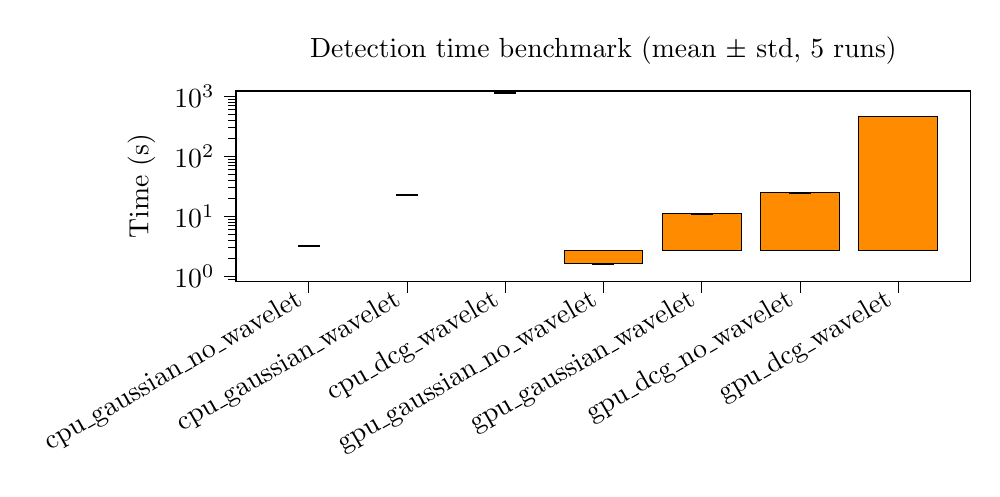
\begin{tikzpicture}

\definecolor{darkgray176}{RGB}{176,176,176}
\definecolor{darkorange}{RGB}{255,140,0}
\definecolor{lightgray204}{RGB}{204,204,204}
\definecolor{steelblue}{RGB}{70,130,180}

\begin{axis}[
height=4cm,
width=0.9\textwidth,
legend cell align={left},
legend style={fill opacity=0.8, draw opacity=1, text opacity=1, draw=lightgray204},
tick align=outside,
tick pos=left,
title={Detection time benchmark (mean ± std, 5 runs)},
x grid style={darkgray176},
xmin=-0.74, xmax=6.74,
xtick style={color=black},
xtick={0,1,2,3,4,5,6},
xticklabel style={rotate=30.0,anchor=east},
xticklabels={
  cpu\_gaussian\_no\_wavelet,
  cpu\_gaussian\_wavelet,
  cpu\_dcg\_wavelet,
  gpu\_gaussian\_no\_wavelet,
  gpu\_gaussian\_wavelet,
  gpu\_dcg\_no\_wavelet,
  gpu\_dcg\_wavelet
},
y grid style={darkgray176},
ylabel={Time (s)},
ymax=1224.04057289162,
ytick style={color=black},
ymode=log
]
\draw[draw=black,fill=darkorange,line width=0.24pt] (axis cs:2.6,0) rectangle (axis cs:3.4,1.61280055962);
\draw[draw=black,fill=darkorange,line width=0.24pt] (axis cs:3.6,0) rectangle (axis cs:4.4,10.98517668238);
\draw[draw=black,fill=darkorange,line width=0.24pt] (axis cs:4.6,0) rectangle (axis cs:5.4,24.66168589718);
\draw[draw=black,fill=darkorange,line width=0.24pt] (axis cs:5.6,0) rectangle (axis cs:6.4,460.99272668412);
\path [draw=black, semithick]
(axis cs:0,3.11705565599688)
--(axis cs:0,3.17154756096312);

\path [draw=black, semithick]
(axis cs:1,22.736708568896)
--(axis cs:1,23.016265406904);

\path [draw=black, semithick]
(axis cs:2,1140.36295115439)
--(axis cs:2,1165.75292656345);

\path [draw=black, semithick]
(axis cs:3,1.59673847648965)
--(axis cs:3,1.62886264275035);

\path [draw=black, semithick]
(axis cs:4,10.9241175710869)
--(axis cs:4,11.0462357936732);

\path [draw=black, semithick]
(axis cs:5,24.5458291466455)
--(axis cs:5,24.7775426477145);

\path [draw=black, semithick]
(axis cs:6,460.326750349203)
--(axis cs:6,461.658703019037);

\addplot [semithick, black, mark=-, mark size=4, mark options={solid}, only marks, forget plot]
table {%
0 3.11705565599688
1 22.736708568896
2 1140.36295115439
3 1.59673847648965
4 10.9241175710869
5 24.5458291466455
6 460.326750349203
};
\addplot [semithick, black, mark=-, mark size=4, mark options={solid}, only marks, forget plot]
table {%
0 3.17154756096312
1 23.016265406904
2 1165.75292656345
3 1.62886264275035
4 11.0462357936732
5 24.7775426477145
6 461.658703019037
};
\end{axis}

\end{tikzpicture}

  
% This file was created with matplot2tikz v0.5.3.
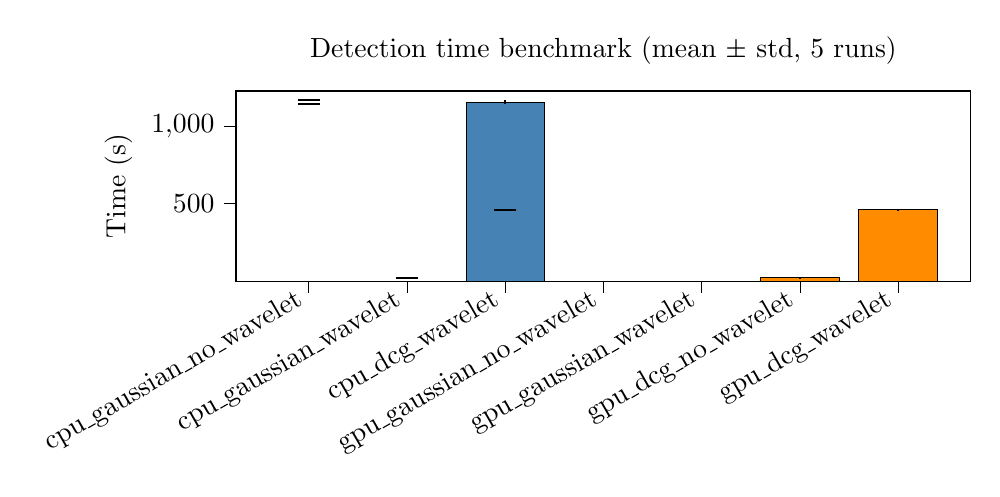
\begin{tikzpicture}

\definecolor{darkgray176}{RGB}{176,176,176}
\definecolor{darkorange}{RGB}{255,140,0}
\definecolor{lightgray204}{RGB}{204,204,204}
\definecolor{steelblue}{RGB}{70,130,180}

\begin{axis}[
height=4cm,
width=0.9\textwidth,
legend cell align={left},
legend style={fill opacity=0.8, draw opacity=1, text opacity=1, draw=lightgray204},
tick align=outside,
tick pos=left,
title={Detection time benchmark (mean ± std, 5 runs)},
x grid style={darkgray176},
xmin=-0.74, xmax=6.74,
xtick style={color=black},
xtick={0,1,2,3,4,5,6},
xticklabel style={rotate=30.0,anchor=east},
xticklabels={
  cpu\_gaussian\_no\_wavelet,
  cpu\_gaussian\_wavelet,
  cpu\_dcg\_wavelet,
  gpu\_gaussian\_no\_wavelet,
  gpu\_gaussian\_wavelet,
  gpu\_dcg\_no\_wavelet,
  gpu\_dcg\_wavelet
},
y grid style={darkgray176},
ylabel={Time (s)},
ymax=1224.04057289162,
ytick style={color=black},
ymin=1,
]
\draw[draw=black,fill=steelblue,line width=0.24pt] (axis cs:1.6,0) rectangle (axis cs:2.4,1153.05793885892);
\draw[draw=black,fill=darkorange,line width=0.24pt] (axis cs:4.6,0) rectangle (axis cs:5.4,24.66168589718);
\draw[draw=black,fill=darkorange,line width=0.24pt] (axis cs:5.6,0) rectangle (axis cs:6.4,460.99272668412);

\path [draw=black, semithick]
(axis cs:2,1140.36295115439)
--(axis cs:2,1165.75292656345);


\path [draw=black, semithick]
(axis cs:5,24.5458291466455)
--(axis cs:5,24.7775426477145);

\path [draw=black, semithick]
(axis cs:6,460.326750349203)
--(axis cs:6,461.658703019037);

\addplot [semithick, black, mark=-, mark size=4, mark options={solid}, only marks, forget plot]
table {%
0 1140.36295115439
1 24.5458291466455
2 460.326750349203
};
\addplot [semithick, black, mark=-, mark size=4, mark options={solid}, only marks, forget plot]
table {%
0 1165.75292656345
1 24.7775426477145
2 461.658703019037
};
\end{axis}

\end{tikzpicture}

  \caption{Comparaison des temps de calculs sur CPU et GPU des cartes de détection de changements sur la Scene 1 avec ($\vdim=12$) ou sans ($\vdim=3$) la décomposition en ondelettes \cite{Mian_wavelet_2019}. Nombre de répétions : 10 (après 5 répétitions de chauffe).}
  \label{fig:benchmark_sar_offline}
\end{figure}



\subsection{Estimation récursive des matrices de covariances structurées par la géométrie riemannienne}

[Provide analysis and discussion of the topics covered in this chapter.]

\section*{Key Insight}
Use kaobox environments to highlight important concepts, definitions, or insights that readers should pay special attention to.

\section{Synthèse}
\label{sec:detection-synthese}


This chapter has covered [summarize the main points]. The key takeaways are:

\begin{enumerate}
    \item First main point or contribution
    \item Second main point or contribution
    \item Third main point or contribution
\end{enumerate}

The next chapter will [preview what comes next].



Lorem ipsum dolor sit amet, consectetur adipiscing elit. Sed vitae viverra nisl. Vivamus nec eleifend lectus. Aenean interdum erat lorem, sed porttitor velit mattis eu. In vel ante quis lacus consectetur dapibus. Vivamus sit amet lorem vitae mauris maximus maximus et at tellus. Aliquam erat volutpat. Suspendisse potenti. Phasellus vel scelerisque felis, ac pellentesque turpis. Donec facilisis erat in ligula tempor, at lacinia nulla accumsan. Sed tincidunt semper ornare. Nulla posuere pretium metus, at aliquet leo aliquet nec. Etiam imperdiet, nunc vitae lobortis ultricies, ligula magna rhoncus sem, non ullamcorper elit odio pellentesque tellus. Etiam euismod pharetra nibh, sed laoreet libero egestas quis. Mauris a eros sed nisi semper pretium. Nam ac ante scelerisque, accumsan odio ut, aliquam lorem. Phasellus ac efficitur est.

Suspendisse sollicitudin arcu non felis tincidunt dignissim. Vestibulum nisi nisl, malesuada vel pretium nec, congue non justo. Praesent varius hendrerit vulputate. Aenean eros ligula, sagittis quis euismod eu, hendrerit sit amet leo. Proin vitae ex consequat, accumsan odio id, maximus leo. Quisque gravida ipsum ac eleifend fermentum. Morbi varius ultricies sollicitudin. Ut in lacus id felis tincidunt tincidunt. Donec rutrum hendrerit placerat. Cras non interdum dolor. Curabitur placerat ut lectus ac ullamcorper. Pellentesque purus tortor, aliquet id elit eget, ultrices egestas eros. Maecenas dapibus eros ex, a accumsan est placerat ac. Donec ac risus justo.

Nam sodales accumsan sem, quis viverra dui tincidunt eu. Proin ac risus vitae felis condimentum viverra. Curabitur sodales bibendum est nec consequat. Sed euismod malesuada venenatis. Aliquam in lorem nulla. Praesent eleifend, velit nec auctor consequat, quam ex tristique risus, eu porttitor elit urna at quam. Nunc lectus lacus, ornare id nisi aliquet, luctus imperdiet libero. In in auctor orci, in ullamcorper nisi. Aliquam fringilla consequat mi eu interdum. Donec enim dolor, facilisis ac dui non, molestie vehicula velit. Integer fermentum fringilla lectus, ut pellentesque est posuere ac. Phasellus purus nunc, fringilla non porttitor sit amet, vehicula id turpis. Duis rutrum imperdiet quam, id laoreet turpis dignissim quis. Donec blandit lobortis sapien.

